\documentclass[a4paper,10pt]{article}
\usepackage[a4paper]{geometry}
\geometry{hscale=0.8,vscale=0.8,centering}
\usepackage[utf8]{inputenc}
\usepackage[T1]{fontenc}
\usepackage[french]{babel} % Exposant


\usepackage{enumerate} % Listes
\usepackage{amsmath} % Matrices
\usepackage{graphicx}
\usepackage{amssymb}
\usepackage{ulem}
\usepackage{color} % Couleurs
\usepackage{fancyvrb} % Couleurs dans Verbatim
\usepackage{subfig} % Sous-figure de figure
\usepackage{listings} % Lecture du code
\usepackage{hyperref} % Hyperlien


% Mise en page spéciale fancyhdr pour les en-têtes
\usepackage{fancyhdr}
\pagestyle{fancy}

\renewcommand{\headrulewidth}{0pt}
\fancyhead[C]{} % Rien en haut de page au milieu
\fancyhead[L]{\leftmark} % Nom du chapitre actuel en haut de page à gauche
\fancyhead[R]{\thepage} % Numéro de page en haut de page à droite

\renewcommand{\footrulewidth}{0pt}
\fancyfoot[C]{Université Libre de Bruxelles} % Rien en bas de page au milieu
\fancyfoot[L]{INFOF203 - Algorithmique 2} % Numéro de page en bas de page à gauche
\fancyfoot[R]{\thepage} % Numéro de page en bas de page à droite
\setlength{\headheight}{12.1638pt}

% Configuration de listings
\definecolor{mygreen}{rgb}{0,0.6,0}
\definecolor{mygray}{rgb}{0.5,0.5,0.5}
\definecolor{mymauve}{rgb}{0.58,0,0.82}

\lstset{ %
  backgroundcolor=\color{white},   % choose the background color; you must add \usepackage{color} or \usepackage{xcolor}
  basicstyle=\footnotesize,        % the size of the fonts that are used for the code
  breakatwhitespace=false,         % sets if automatic breaks should only happen at whitespace
  breaklines=true,                 % sets automatic line breaking
  captionpos=b,                    % sets the caption-position to bottom
  commentstyle=\color{mygreen},    % comment style
  deletekeywords={...},            % if you want to delete keywords from the given language
  escapeinside={\%*}{*)},          % if you want to add LaTeX within your code
  extendedchars=true,              % lets you use non-ASCII characters; for 8-bits encodings only, does not work with UTF-8
  frame=single,                    % adds a frame around the code
  keepspaces=true,                 % keeps spaces in text, useful for keeping indentation of code (possibly needs columns=flexible)
  keywordstyle=\color{blue},       % keyword style
  language=Octave,                 % the language of the code
  morekeywords={*,...},            % if you want to add more keywords to the set
  numbers=left,                    % where to put the line-numbers; possible values are (none, left, right)
  numbersep=5pt,                   % how far the line-numbers are from the code
  numberstyle=\tiny\color{mygray}, % the style that is used for the line-numbers
  rulecolor=\color{black},         % if not set, the frame-color may be changed on line-breaks within not-black text (e.g. comments (green here))
  showspaces=false,                % show spaces everywhere adding particular underscores; it overrides 'showstringspaces'
  showstringspaces=false,          % underline spaces within strings only
  showtabs=false,                  % show tabs within strings adding particular underscores
  stepnumber=1,                    % the step between two line-numbers. If it's 1, each line will be numbered
  stringstyle=\color{mymauve},     % string literal style
  tabsize=2,                       % sets default tabsize to 2 spaces
  %title=\lstname                   % show the filename of files included with \lstinputlisting; also try caption instead of title
}


\author{Rodrigue \textsc{Van Brande}} % Auteur
\date{\today} % Date de compilation du pdf

\pdfinfo{
    /Author   (Rodrigue VAN BRANDE)
    /Creator  (LaTeX)
}

%Création d'un subsub...section (avec \paragraph{} \subparagraph{})
\setcounter{secnumdepth}{5}
\setcounter{tocdepth}{5}


%\newcommand{\fonction}[nb de parametre]{définition de la commande}
\newcommand{\guillemets}[1]{\og #1 \fg} % citation entre guillemets
\newcommand{\gras}[1]{\textbf{#1}} %met en gras
\newcommand{\italique}[1]{\textit{#1}} %met en italique

% Titre du PDF
\title{INFOF203 - Algorithmique 2\\Rapport}

% Propriété du PDF
\pdfinfo{
/Title{INFOF203 - Algorithmique 2 - Rapport}
}

%Profondeur pour la table des matières dans les titres
\setcounter{tocdepth}{3}

\begin{document}
	\maketitle       %Titre
	\newpage         %Saut de page
	\tableofcontents %table des matières / Besoin d'une double compilation
	\newpage         %Saut de page

	\section{Arbre binaire}

Le labyrinthe est une simple matrice où chaque élément est une \textit{Case}. Mais on peut aussi le décomposer en un arbre binaire car le labyrinthe imposé dans le projet est dit "parfait" \footnote{Cette notion a été reprise de $\href{http://fr.wikipedia.org/wiki/Mod\%C3\%A9lisation_math\%C3\%A9matique_d\%27un_labyrinthe}{fr.wikipedia}$.}.

\begin{figure}[!h]
  \centering
  \subfloat[Un labyrinthe parfait contenant son arbre.]{\label{fig:edge-a}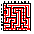
\includegraphics[width=0.4\textwidth]{4.arbreBinaire/maze.pdf}}
  \hspace{5pt}
  \subfloat[Représentation en arbre du labyrinthe.]{\label{fig:contour-b}
\includegraphics[width=0.4\textwidth]{4.arbreBinaire/tree.pdf}}
  \hspace{5pt}
  \caption{Le labyrinthe et son arbre associé.}
\end{figure}

Cette arbre est donc construit par la classe \textit{Path} sous forme de plusieurs \textit{Tree} comme vu au cours.
    \section{Arbre binaire}

Le labyrinthe est une simple matrice où chaque élément est une \textit{Case}. Mais on peut aussi le décomposer en un arbre binaire car le labyrinthe imposé dans le projet est dit "parfait" \footnote{Cette notion a été reprise de $\href{http://fr.wikipedia.org/wiki/Mod\%C3\%A9lisation_math\%C3\%A9matique_d\%27un_labyrinthe}{fr.wikipedia}$.}.

\begin{figure}[!h]
  \centering
  \subfloat[Un labyrinthe parfait contenant son arbre.]{\label{fig:edge-a}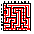
\includegraphics[width=0.4\textwidth]{4.arbreBinaire/maze.pdf}}
  \hspace{5pt}
  \subfloat[Représentation en arbre du labyrinthe.]{\label{fig:contour-b}
\includegraphics[width=0.4\textwidth]{4.arbreBinaire/tree.pdf}}
  \hspace{5pt}
  \caption{Le labyrinthe et son arbre associé.}
\end{figure}

Cette arbre est donc construit par la classe \textit{Path} sous forme de plusieurs \textit{Tree} comme vu au cours.
    \section{Arbre binaire}

Le labyrinthe est une simple matrice où chaque élément est une \textit{Case}. Mais on peut aussi le décomposer en un arbre binaire car le labyrinthe imposé dans le projet est dit "parfait" \footnote{Cette notion a été reprise de $\href{http://fr.wikipedia.org/wiki/Mod\%C3\%A9lisation_math\%C3\%A9matique_d\%27un_labyrinthe}{fr.wikipedia}$.}.

\begin{figure}[!h]
  \centering
  \subfloat[Un labyrinthe parfait contenant son arbre.]{\label{fig:edge-a}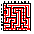
\includegraphics[width=0.4\textwidth]{4.arbreBinaire/maze.pdf}}
  \hspace{5pt}
  \subfloat[Représentation en arbre du labyrinthe.]{\label{fig:contour-b}
\includegraphics[width=0.4\textwidth]{4.arbreBinaire/tree.pdf}}
  \hspace{5pt}
  \caption{Le labyrinthe et son arbre associé.}
\end{figure}

Cette arbre est donc construit par la classe \textit{Path} sous forme de plusieurs \textit{Tree} comme vu au cours.
    \section{Arbre binaire}

Le labyrinthe est une simple matrice où chaque élément est une \textit{Case}. Mais on peut aussi le décomposer en un arbre binaire car le labyrinthe imposé dans le projet est dit "parfait" \footnote{Cette notion a été reprise de $\href{http://fr.wikipedia.org/wiki/Mod\%C3\%A9lisation_math\%C3\%A9matique_d\%27un_labyrinthe}{fr.wikipedia}$.}.

\begin{figure}[!h]
  \centering
  \subfloat[Un labyrinthe parfait contenant son arbre.]{\label{fig:edge-a}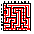
\includegraphics[width=0.4\textwidth]{4.arbreBinaire/maze.pdf}}
  \hspace{5pt}
  \subfloat[Représentation en arbre du labyrinthe.]{\label{fig:contour-b}
\includegraphics[width=0.4\textwidth]{4.arbreBinaire/tree.pdf}}
  \hspace{5pt}
  \caption{Le labyrinthe et son arbre associé.}
\end{figure}

Cette arbre est donc construit par la classe \textit{Path} sous forme de plusieurs \textit{Tree} comme vu au cours.
    \section{Arbre binaire}

Le labyrinthe est une simple matrice où chaque élément est une \textit{Case}. Mais on peut aussi le décomposer en un arbre binaire car le labyrinthe imposé dans le projet est dit "parfait" \footnote{Cette notion a été reprise de $\href{http://fr.wikipedia.org/wiki/Mod\%C3\%A9lisation_math\%C3\%A9matique_d\%27un_labyrinthe}{fr.wikipedia}$.}.

\begin{figure}[!h]
  \centering
  \subfloat[Un labyrinthe parfait contenant son arbre.]{\label{fig:edge-a}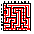
\includegraphics[width=0.4\textwidth]{4.arbreBinaire/maze.pdf}}
  \hspace{5pt}
  \subfloat[Représentation en arbre du labyrinthe.]{\label{fig:contour-b}
\includegraphics[width=0.4\textwidth]{4.arbreBinaire/tree.pdf}}
  \hspace{5pt}
  \caption{Le labyrinthe et son arbre associé.}
\end{figure}

Cette arbre est donc construit par la classe \textit{Path} sous forme de plusieurs \textit{Tree} comme vu au cours.

\end{document}
